\documentclass{beamer}
\usetheme{Boadilla}

\usefonttheme{serif}

\usepackage{subfigure}
\usepackage{latexsym,amsmath,amssymb}
\usepackage[natbibapa]{apacite}
\usepackage{algorithm}
\usepackage{algorithmic}
\usepackage{graphicx}
\usepackage{times}
\usepackage[section]{placeins}
\usepackage{listings}
\usepackage{bm}
\usepackage[retainorgcmds]{IEEEtrantools}
\usepackage[showonlyrefs]{mathtools}
\usepackage{hyperref}
\usepackage{tabu}

\title{Learning our ABCs}

\author{Nathan Cunningham \and Sherman Ip \and Ella Kaye}

\date{February 12th, 2016}

\begin{document}

\begin{frame}
\maketitle
\centering
\includegraphics{ABC_blocks}
\end{frame}

\begin{frame}
\frametitle{Outline}
\begin{itemize}
\item Approximate Bayesian computation
\item ABC with conjugate priors
\item ABC and semi-automatic ABC with the g-and-k distribution
\end{itemize}
\end{frame}

\begin{frame}
\frametitle{Background and Motivation}
\begin{block}{Full Posterior}
\[
\pi(\theta | y_{obs}) = \frac{p(y_{obs} | \theta) \pi(\theta)}{p(y_{obs})}
\]
\end{block}
\pause
\begin{block}{Partial Posterior}
\[
\pi(\theta | s_{obs}) = \frac{p(s_{obs} | \theta) \pi(\theta)}{p(s_{obs})}
\]
where $s_{obs} = S(y_{obs})$ is a vector of summary statistics (preferably sufficient) of lower dimension than the data
\end{block}
\end{frame}

\begin{frame}
\frametitle{ABC approximation (rejection algorithm)}
$\pi_{\epsilon}(\theta | y_{obs})$, is generated by repeatedly

\begin{itemize}
\item Generating $\theta'$ from the prior distribution $\pi(\cdot)$
\item Generating $y_i$ from the likelihood $p(\cdot | \theta')$
\item Accepting $\theta'$ if $\rho\{S(y_i), S(y_{obs})\} \leq \epsilon$
\end{itemize}
\pause
Requires tuning of 
\begin{itemize}
\item $S(\cdot)$, the function to compute summary statistics
\item $\rho$, the distance function
\item $\epsilon$, the threshold
\end{itemize}
\end{frame}

\begin{frame}
\frametitle{ABC with local linear regression...}
\begin{itemize}
\item Improve the previous algorithm by introducing a regression step to correct for discrepancy between $S(y_{obs})$ and $S(y_i)$
\item For each simulated $y_i$, set
\[
\theta_i = m(S(y_i)) + \eta_i
\]
where $m$ is the regression function and the $\eta_i$ are centered random variables with common variance. 
\end{itemize}
\end{frame}

\begin{frame}
\frametitle{...and kernel}
\begin{itemize}
\item Instead of accepting or rejecting a sample, assign each simulation $(\theta_i, S(y_i))$ a weight with a kernel
\[
K[\rho(S(y_i), S(y_{obs}))]
\]
\item Higher weights given for proximity to the observation
\item We use the Epanechnikov kernel and the Euclidean distance function
\end{itemize}
\end{frame}

\begin{frame}
\frametitle{Principled summary statistic selection}
\begin{itemize}
\item Best subset selection
\pause
\item Semi-automatic ABC
\begin{enumerate}
\item Inital run of ABC to find a posterior region of non-negligible mass
\item Simulate parameter values and summary statistics
\item Run a linear regression of the summary statistics on each parameter. Use an information criterion such as BIC to determine which summary statistics can best be used to infer the parameter values
\item Run ABC using this choice of summary statistics
\end{enumerate}
\end{itemize}
\end{frame}

\begin{frame}
\frametitle{Beta prior, binomial likelihood}
\begin{equation}
\theta\sim\textup{Beta}(1,1)
\end{equation}
\begin{equation}
X|\theta\sim\textup{Bin}(12,\theta)
\end{equation}
\begin{equation}
\theta|X=2\sim\textup{Beta}(3,11)
\end{equation}
\pause
\begin{block}{ABC Algorithm}
\begin{itemize}
  \item Sample $\theta\sim\textup{Beta}(1,1)$
  \item Sample $X|\theta\sim\textup{Bin}(12,\theta)$
  \item Accept $\theta$ if $X|\theta = 2$, otherwise reject.
\end{itemize}
\end{block}
\end{frame}

\begin{frame}
\frametitle{Beta prior, binomial likelihood}
\begin{figure}
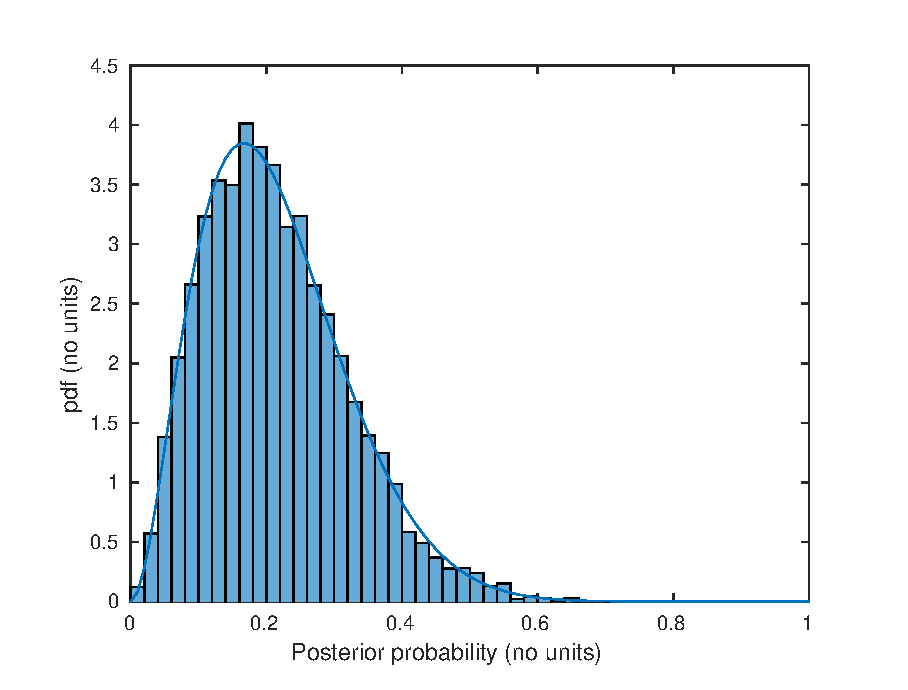
\includegraphics[width=0.5\textwidth]{binomial_ABC0528.eps}
\caption{10,000 samples using ABC.}
\label{binomial}
\end{figure}
$p$ value for $\chi^2$ goodness of fit test $(50\pm30)\%$ \\
$(10\pm10)$ rejects per accepted sample
\end{frame}

\begin{frame}
\frametitle{Normal-gamma prior, Normal likelihood}
\begin{block}{Prior}
\begin{equation}
\tau\sim\textup{Gamma}(\alpha_0,\beta_0)
\end{equation}
\begin{equation}
\mu|\tau\sim\textup{N}\left(\mu_0,1/(\nu_0\tau)\right)
\end{equation}
\end{block}
\pause
\begin{block}{Likelihood}
\begin{equation}
X|\mu,\tau\sim\textup{N}(\mu,1/\tau)
\end{equation}
\end{block}
\pause
\begin{block}{Joint Posterior}
\begin{equation}
\mu,\tau|X\sim\textup{NGamma}
\left(
	\mu_1,
	\nu_1,
	\alpha_1,
	\beta_1
\right)
\end{equation}
\end{block}

\end{frame}

\begin{frame}
\frametitle{Normal-gamma prior, Normal likelihood}
\begin{block}{Marginal Posterior}
\begin{equation}
\mu|X = \sqrt{\dfrac{\beta_1}{\alpha_1\nu_1}} T_{2\alpha_1}
+ \mu_1
\end{equation}
and
\begin{equation}
\tau|X \sim \textup{Gamma}\left(
\alpha_1,\beta_1
\right)
\end{equation}
where $T_{2\alpha}\sim t_{2\alpha}$.
\end{block}
\end{frame}

\begin{frame}
\frametitle{Normal-gamma prior, Normal likelihood}
\begin{block}{ABC Algorithm}
\begin{itemize}
	\item Sample $\tau\sim\textup{Gamma}(\alpha_0,\beta_0)$
	\item Sample $\mu|\tau\sim\textup{N}\left(\mu_0,1/(\nu_0\tau)\right)$
	\item Sample $n$ times $Y|\mu,\tau\sim\textup{N}(\mu,1/\tau)$
	\pause
	\item Conduct two tailed hypothesis tests, at some confidence level, on
	\begin{equation}
	\dfrac{\sqrt{n}\left(\bar{X}-\bar{Y}\right)}{\sqrt{S_X^2+S_Y^2}}\sim\textup{N}(0,1)
	\end{equation}
	\begin{equation}
	\dfrac{S_X^2}{S_Y^2}\sim F_{n-1,n-1}
	\end{equation}
	\item Accept $\mu,\tau$ if both null hypothesis are accepted, reject otherwise
\end{itemize}
\end{block}
\end{frame}

\begin{frame}
\frametitle{Normal-gamma prior, Normal likelihood}
\begin{figure}
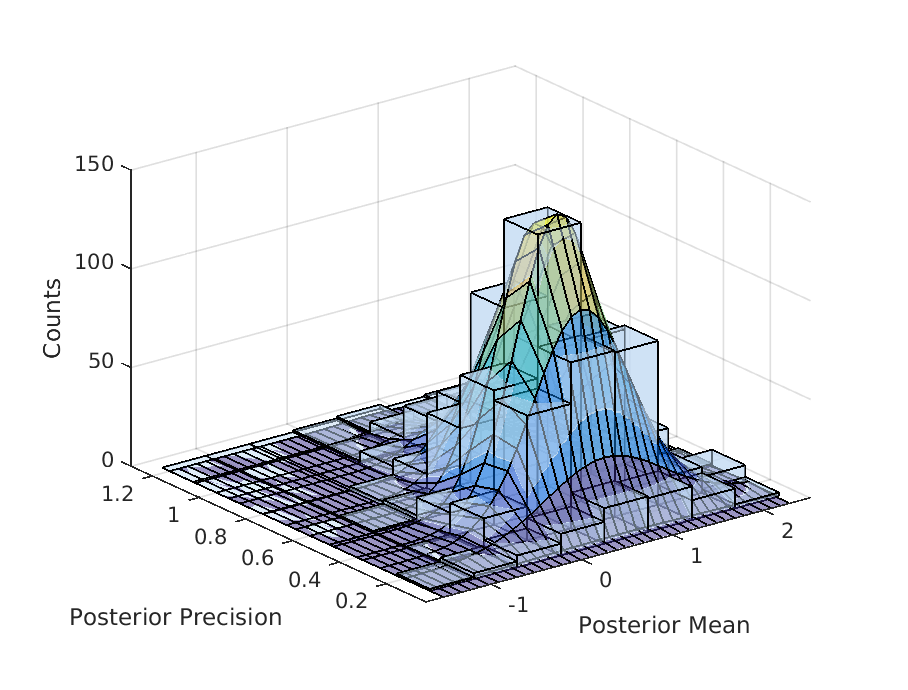
\includegraphics[width=0.5\textwidth]{surf.eps}
\caption{Joint histogram of 1000 samples from ABC. Confidence level set at $10\%$.}
\label{surf}
\end{figure}
\end{frame}

\begin{frame}
\frametitle{Normal-gamma prior, Normal likelihood}
\begin{figure}
\centering
\begin{subfigure}
\centering
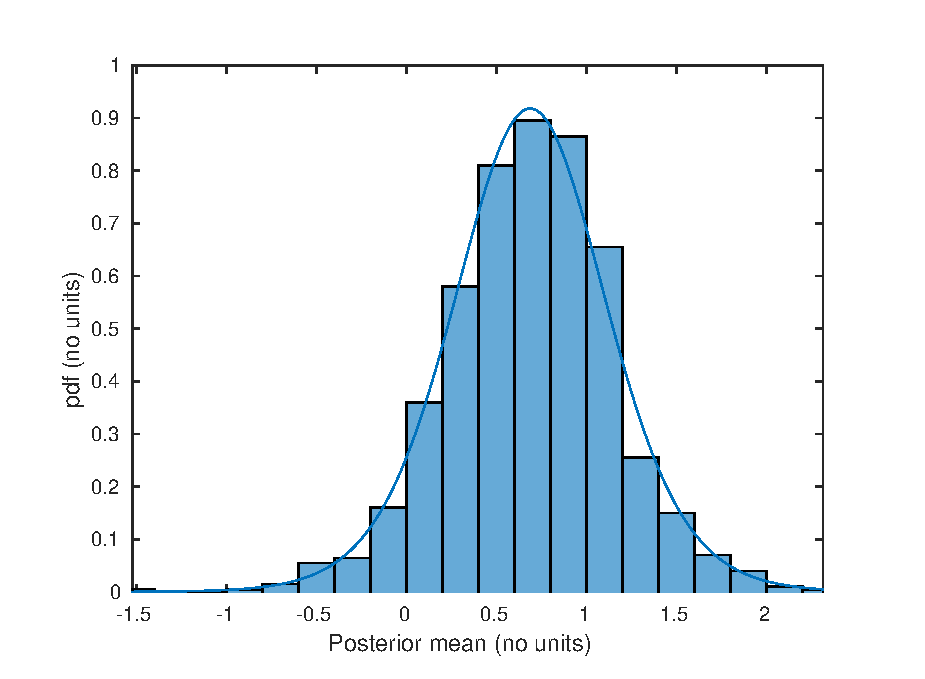
\includegraphics[width=0.45\textwidth]{mean.eps}
\end{subfigure}
\begin{subfigure}
\centering
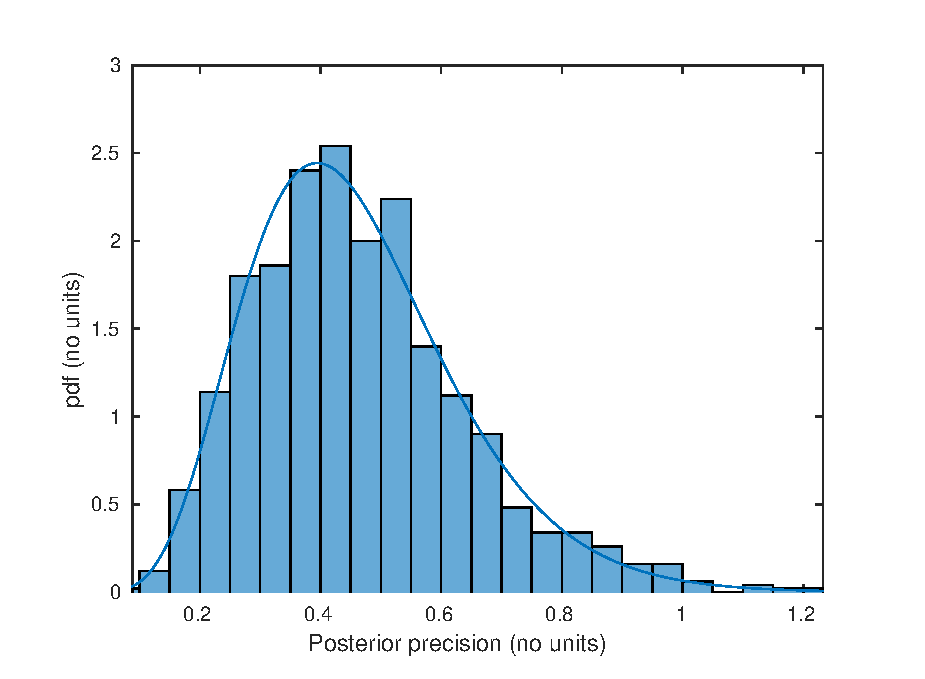
\includegraphics[width=0.45\textwidth]{precision.eps}
\end{subfigure}
\caption{Marginal histogram of 100- samples from ABC. Confidence level set at $10\%$.}
\end{figure}
\end{frame}

\begin{frame}
\frametitle{Normal-gamma prior, Normal likelihood}
\begin{figure}
\centering
\begin{subfigure}
\centering
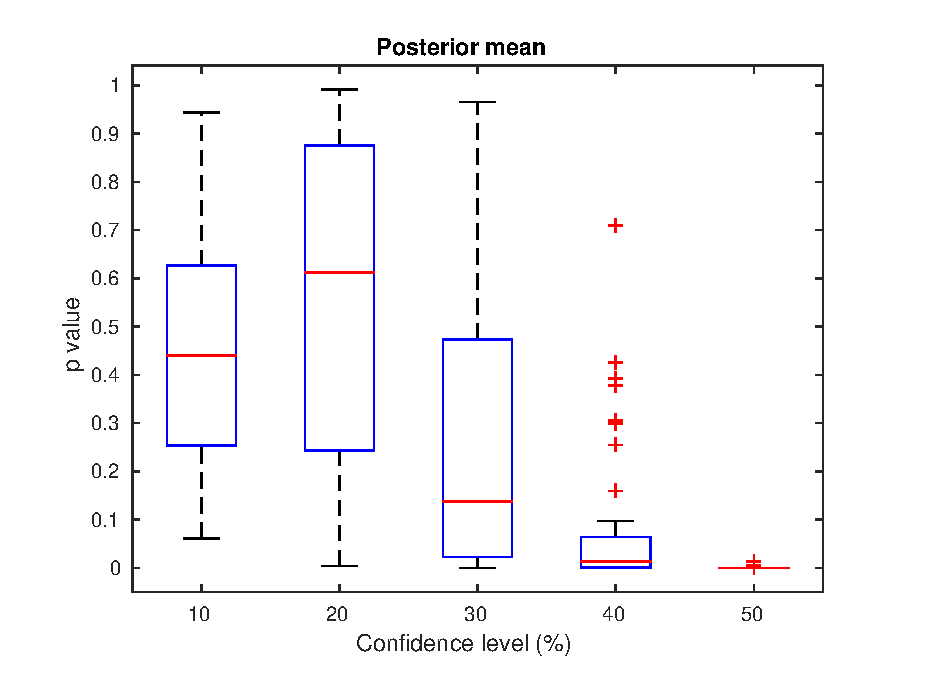
\includegraphics[width=0.45\textwidth]{pvalue_mean.eps}
\end{subfigure}
\begin{subfigure}
\centering
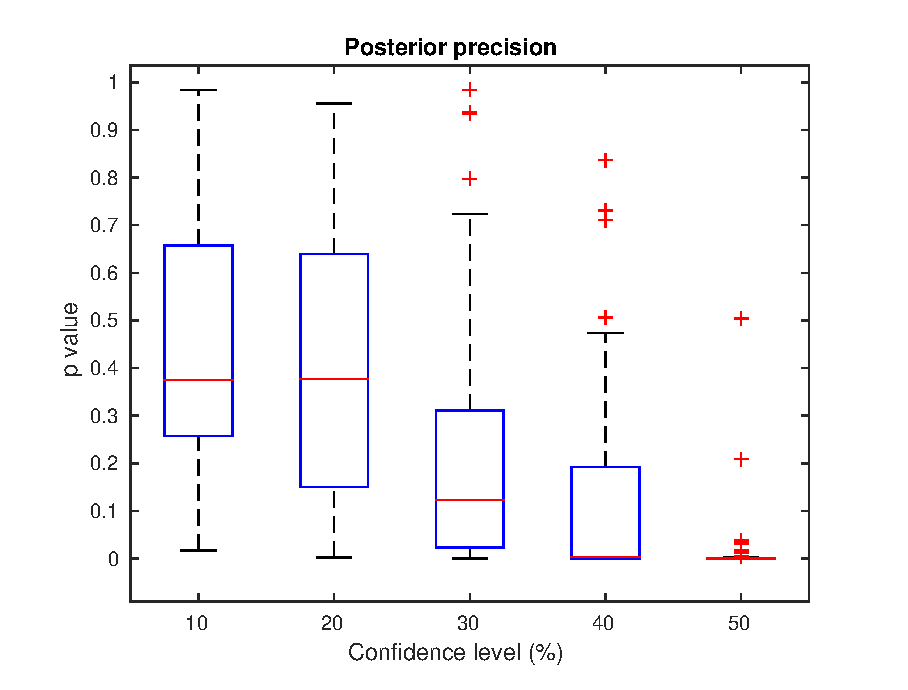
\includegraphics[width=0.45\textwidth]{pvalue_precision.eps}
\end{subfigure}
\caption{$p$ values for the $\chi^2$ goodness of fit test. The test was conducted 50 times with different observations.}
\end{figure}
\end{frame}

\begin{frame}
\frametitle{Normal-gamma prior, Normal likelihood}
\begin{figure}
\centering
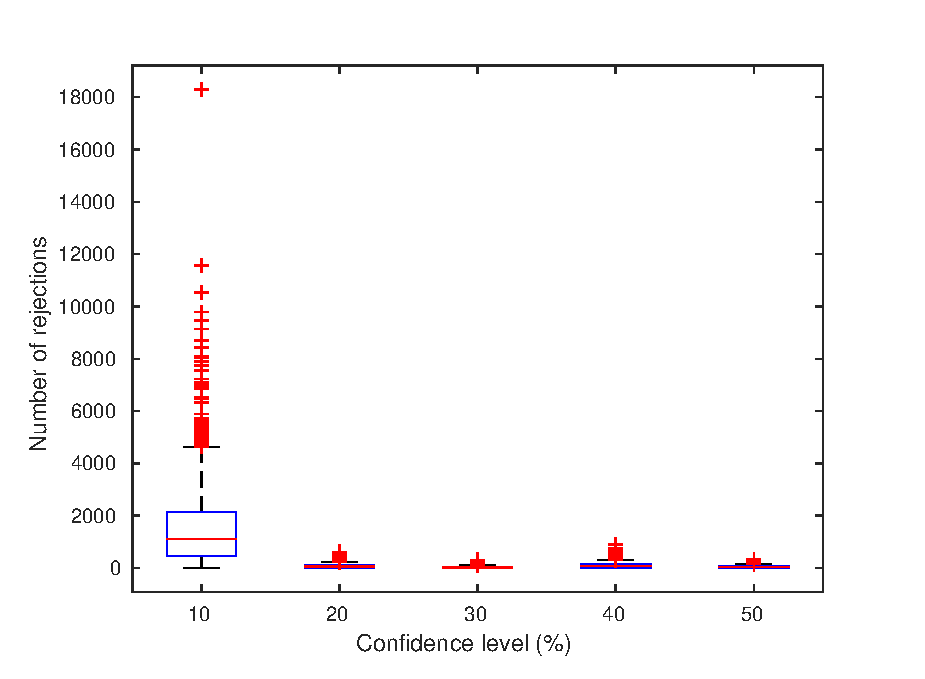
\includegraphics[width=0.45\textwidth]{rejections.eps}
\caption{Rejections per accepted sample}
\end{figure}
\end{frame}

\begin{frame}
\begin{itemize}
\item Threshold not too big, not too small.
\item Ideally comparison through sufficient statistics.
\item Posterior can be unknown.
\item Unable to simulate from improper priors.
\end{itemize}
\end{frame}

\begin{frame}
\frametitle{$g$-and-$k$ distribution}
\begin{itemize}
\item Easy to simulate from, but evaluating likelihood can be costly 
\[
F^{-1}(x, \theta) = A + B\left(1 + c\frac{1-exp(-g.z(x)}{1+exp(-g.z(x)}\right)(1+z(x)^2)^kz(x)
\]
\item $\theta = (A, B, c, g, k)$
\item $c$ taken as fixed at $0.8$
\item Suitable choice of summary statistics not immediately obvious

\end{itemize}
\end{frame}

\begin{frame}
\frametitle{Simulating data}
\begin{itemize}
\item Generate $10^4$ `observations' under `true' $\theta = (A = 3, B = 1, g = 2, k = 0.5)$
\item Simulate $10^5$ parameters from $\mathcal{U}[0,10]^4$
\item Simulate $10^4$ observations from $g$-and-$k$ distribution for each simulated parameter vector
\item Use order statistics as summary statistics
\end{itemize}
\end{frame}

\begin{frame}
\frametitle{Summary statistic selection}
\begin{table}[h]
\centering
\label{tab:bic}
  $\begin{tabu}{| l | l| r|}
  \hline			
    m & l  & mean \\
    \hline
  60 & 1 	& 24,016 \\
  60 & 2  	& 9,470  \\
  60 & 3 	& 1,090 \\
  \mathbf{60} & \mathbf{4} 	& \mathbf{-5,794}\\
  \hline
  100 & 1 	&  25,253 \\
  100 & 2  	&  10,835 \\
  100 & 3 	&  2,946 \\
  100 & 4 	&  -3,447 \\
  \hline
  140 & 1 	 & 24,813  \\
  140 & 2 	 & 10,965 \\
  140 & 3 	 & 3,360  \\
  140 & 4 	& -2,734 \\
  \hline 
  \end{tabu} $
    \caption{The BIC resulting from inferring the parameter values from the order statistics for a variety of number of order statistics ($m$), and powers of these ($l$)}
\end{table}
\end{frame}

\begin{frame}
\frametitle{Fitted vs true parameter values}
\begin{figure}
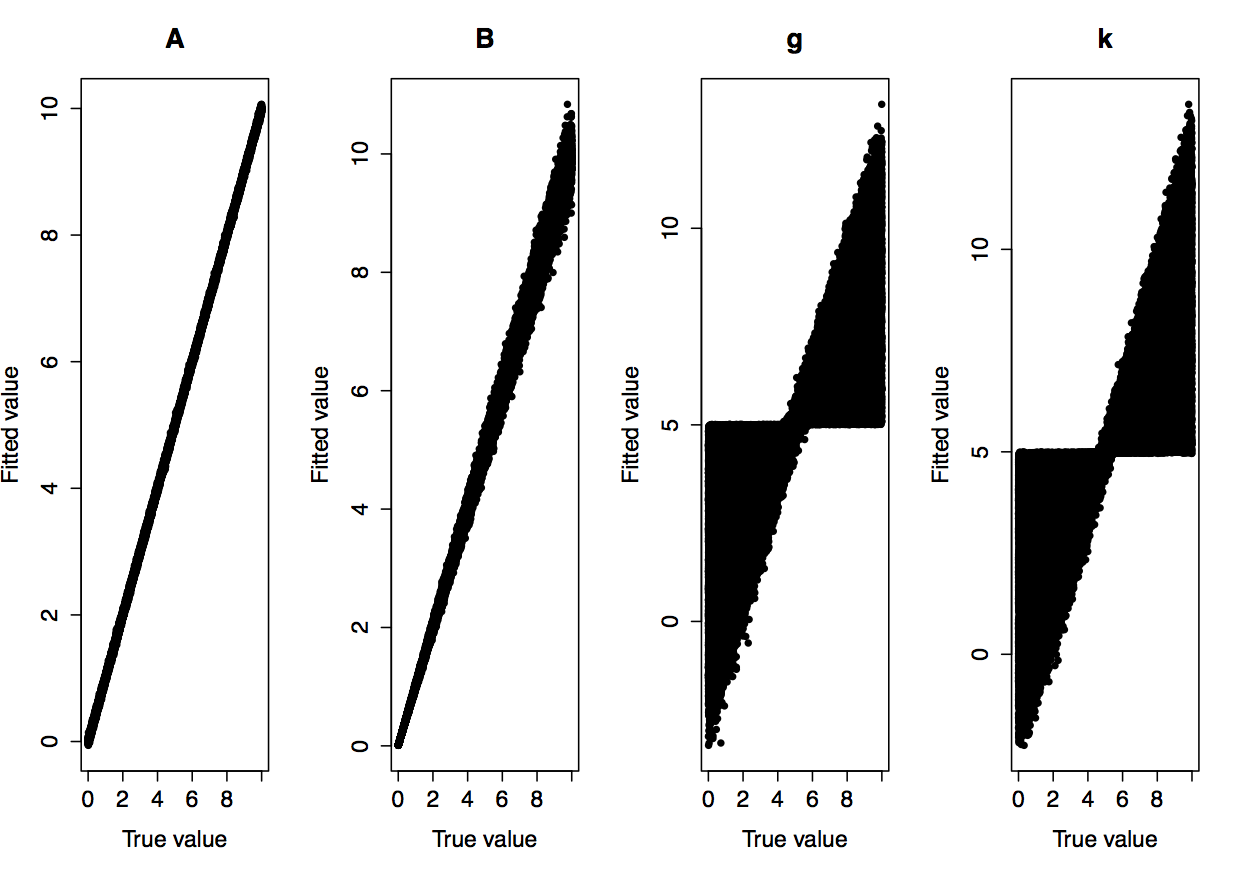
\includegraphics[width = \linewidth, height=2.5in]{firstorder.png}
\caption{Inference of parameter values using order statistics $s$}
\end{figure}
\end{frame}

\begin{frame}
\frametitle{Fitted vs true parameter values}
\begin{figure}
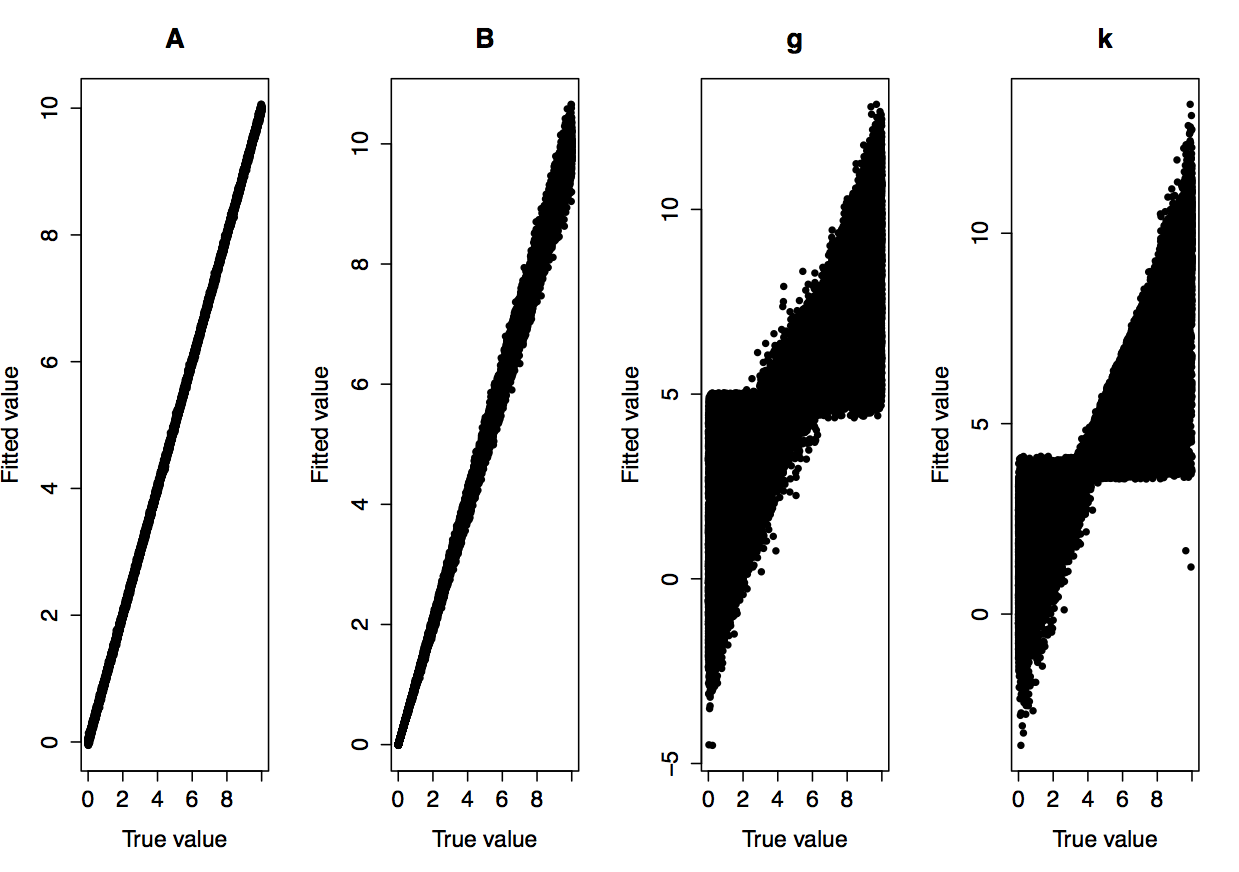
\includegraphics[width = \linewidth, height=2.5in]{fourthorder.png}
\caption{Inference of parameter values using order statistics on summary statistics and transformations $(s, s^2, s^3, s^4)$}
\end{figure}
\end{frame}


\begin{frame}
\frametitle{Inference on A and B parameters}
\begin{figure}
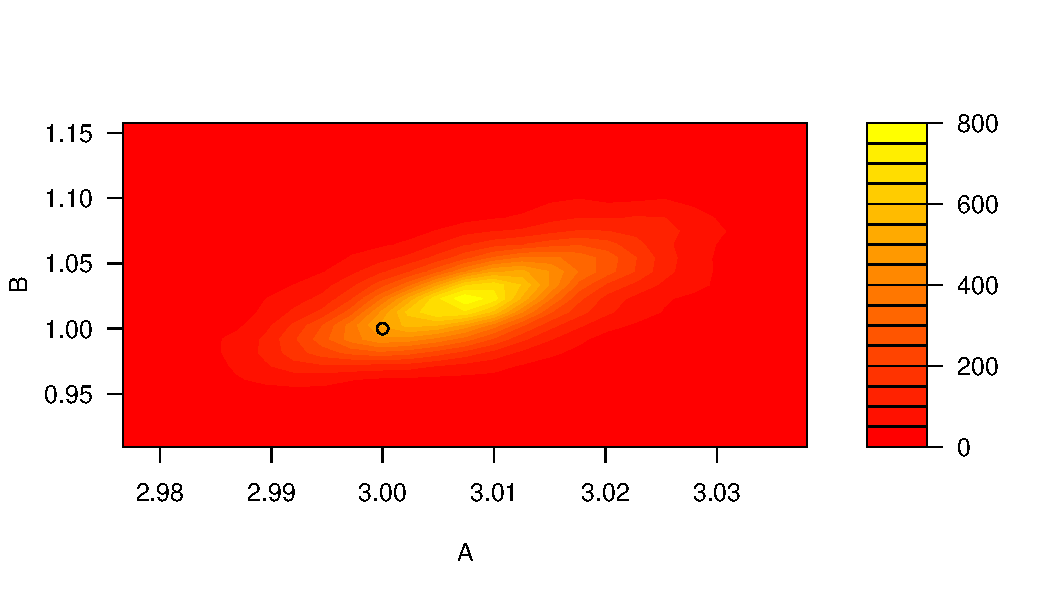
\includegraphics[width = \linewidth]{GK_REG_M_CONT_AB_SA.pdf}
\caption{ABC with semi-automatic summary statistic selection, local linear regresson correction, tolerance 0.01 (chosen by cross-validation)}
\end{figure}
\end{frame}

\begin{frame}
\frametitle{Inference on g and k parameters}
\begin{figure}
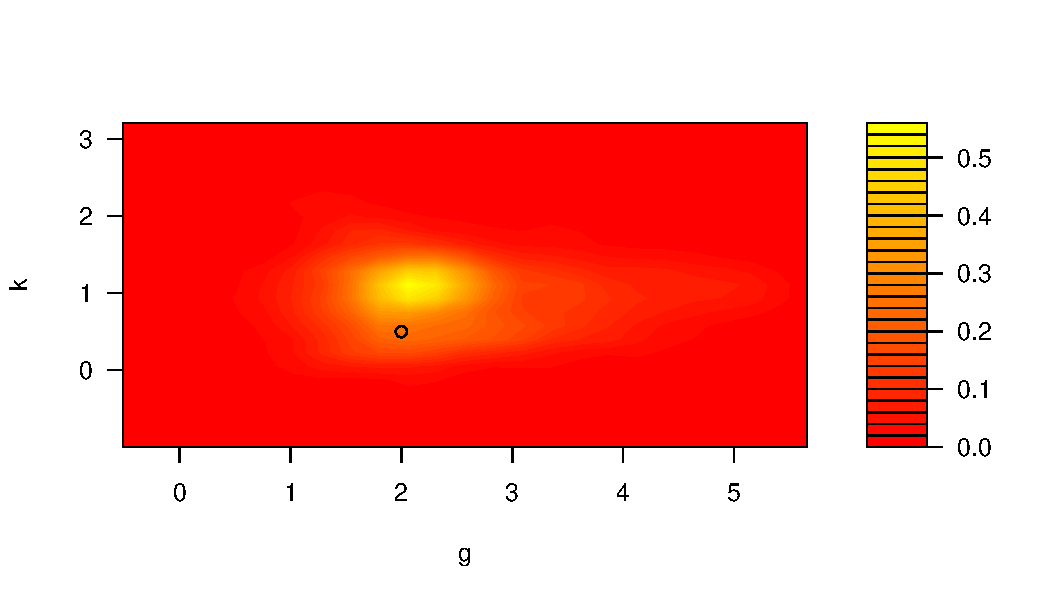
\includegraphics[width = \linewidth]{GK_REG_M_CONT_GK_SA.pdf}
\caption{ABC with semi-automatic summary statistic selection, local linear regresson correction, tolerance 0.01 (chosen by cross-validation)}
\end{figure}
\end{frame}

\begin{frame}
\frametitle{Inference on all parameters}
\begin{figure}
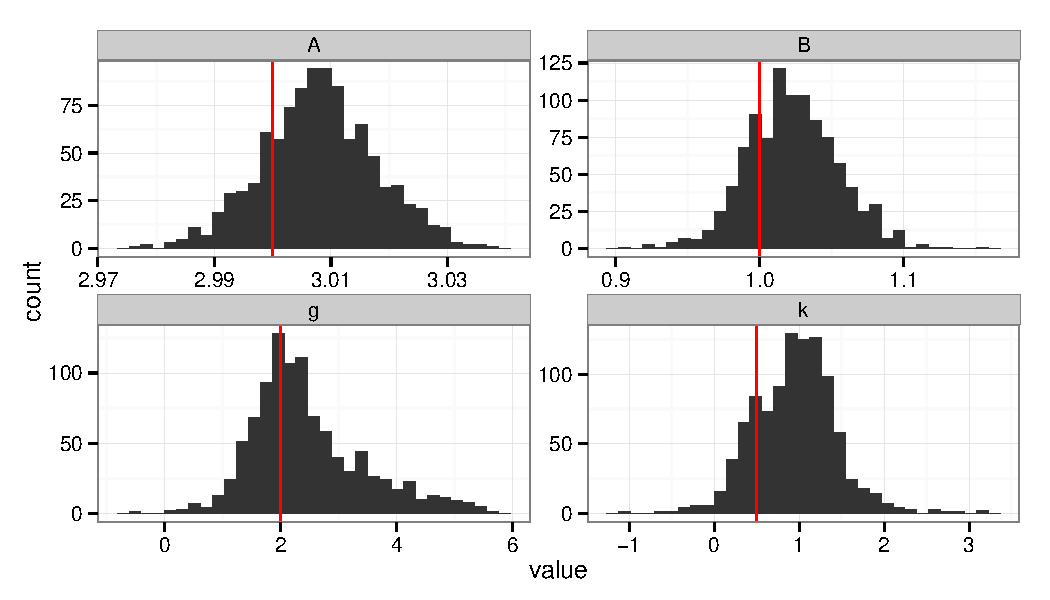
\includegraphics[width = \linewidth]{GK_REG_M_HIST_SA.pdf}
\caption{ABC with semi-automatic summary statistic selection, local linear regresson correction, tolerance 0.01 (chosen by cross-validation)}
\end{figure}
\end{frame}

\begin{frame}
\frametitle{Comparison with standard ABC}
\begin{figure}
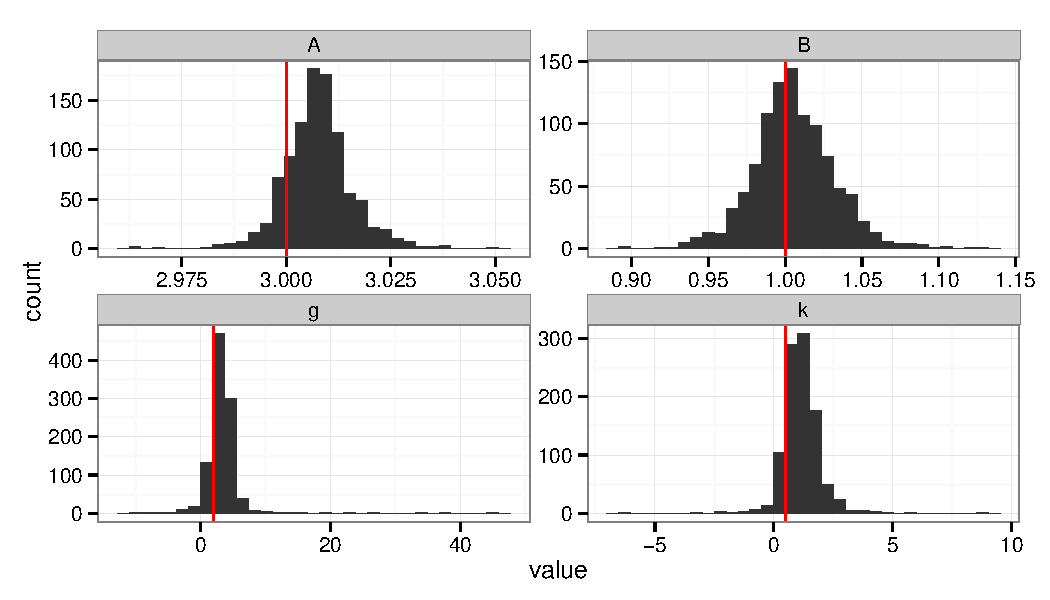
\includegraphics[width = \linewidth]{GK_REG_M_HIST.pdf}
\caption{ABC using 60 order statistics as summary statistics, local linear regresson correction, tolerance 0.01 (chosen by cross-validation)}
\end{figure}
\end{frame}

\begin{frame}
\frametitle{Conclusions}
\begin{itemize}
\item Semi-automatic selection of summary statistics can be useful
\item Not a panacea
\begin{itemize}
\item Still need to choose summary statistics for step 1 
\item Need to choose set of explanatory variables for linear model
\item Still need to tune $\epsilon$, $\rho$ (and $K$)
\end{itemize} 
\item Plenty more to explore \ldots (over to Paul, Giuseppe and Marcin)
\end{itemize}
\end{frame}


\end{document}
